% !TeX root = ../main.tex
\section{Drifting Models for Generation}
\label{sec:methodology}

We propose Drifting Models, which formulate generative modeling as a \emph{training-time} evolution of the pushforward distribution via a drifting field.
Our model naturally performs one-step generation at inference time.

\subsection{Pushforward at Training Time}
\label{subsec:training_time_pushforward}

Consider a neural network $f: \mathbb{R}^C \mapsto \mathbb{R}^D$. The input of $f$ is $\e \sim p_{\e}$ (\eg, any noise of dimension $C$), and the output is denoted by $\x = f(\e) \in \mathbb{R}^D$. In general, the input and output dimensions need not be equal.

We denote the distribution of the network output by $q$, \ie, $\x = f(\e) \sim q$.
In probability theory, $q$ is referred to as the \textit{pushforward} distribution of $p_\e$ under $f$, denoted by:
\begin{equation}
q = f_{\#}p_\e.
\end{equation}
Here, ``$f_{\#}$" denotes the pushforward induced by $f$.
Intuitively, this notation means that $f$ transforms a distribution $p_{\e}$ into another distribution $q$.
The goal of generative modeling is to find $f$ such that $f_{\#}p_{\e} \approx p_\text{data}$.

Since neural network \textit{training} is inherently iterative (\eg, SGD), the training process produces a sequence of models $\{f_i\}$, where $i$ denotes the training iteration.
This corresponds to a sequence of pushforward distributions $\{q_i\}$ during training, where
$q_i = [f_i]_{\#}p_{\e}$ for each $i$.
The training process progressively evolves $q_i$ to match $p_{\text{data}}$.

When the network $f$ is updated,
a sample at training iteration $i$ is implicitly ``drifted'' as:
$\x_{i+1} = \x_{i} + \Delta\x_{i}$, where $ \Delta\x_{i}:=f_{i+1}(\e) - f_{i}(\e)$ arises from parameter updates to $f$.
This implies that the update of $f$ determines the ``\textit{residual}'' of $\x$, which we refer to as the ``drift''.

\subsection{Drifting Field for Training}
\label{subsec:training_objective}

Next, we define a \emph{\textbf{drifting field}} to govern the training-time evolution of the samples $\x$ and, consequently, the pushforward distribution $q$.
A drifting field is a function that computes $ \Delta\x$ given $\x$. Formally, denoting this field by $\V_{p,q}(\cdot)\colon \R^d \to \R^d$, we have: 
\begin{equation}
\x_{i+1}=\x_i+\V_{p,q_i}(\x_i),
\end{equation}
Here, $\x_i=f_i(\e) \sim q_i$ and after drifting we denote $\x_{i+1}\sim q_{i+1}$.
The subscripts $p,q$ denote that this field depends on $p$ (\eg, $p=p_\text{data}$) and the current distribution $q$.

Ideally, when $p=q$, we want all $\x$ to stop drifting \ie, $\V=\textbf{0}$.
In this paper, we consider the following proposition:
\begin{proposition}
Consider an \textbf{anti-symmetric} drifting field:
\begin{equation}
\label{eq:asym}
\V_{p,q}(\x) = - \V_{q,p}(\x),\quad \forall \x.
\end{equation}
Then we have: $\quad q=p \quad \Rightarrow \quad \V_{p,q}(\x) = \mathbf{0},\forall \x$.
\end{proposition}

The proof is straightforward\footnotemark.
Intuitively, anti-symmetry means that swapping $p$ and $q$ simply flips the sign of the drift.
This proposition implies that if the pushforward distribution $q$ matches the data distribution $p$, the drift is zero for any sample and the model achieves an equilibrium.

\footnotetext{$q{=}p \Rightarrow \V_{p,q}{=}\V_{q,p}{=}{-}\V_{p,q} \Rightarrow \V_{p,q}{=}\textbf{0}$}

We note that the converse implication, \ie, $\V_{p,q}=\mathbf{0}\Rightarrow q=p$, is false in general for arbitrary choices of $\V$.
For our kernelized formulation (Sec.~\ref{subsec:instantiation_field}), we give sufficient conditions under which $\V_{p,q}\approx\mathbf{0}$ implies $q\approx p$ (Appendix~\ref{sec:theory_identifiability}).



\paragraph{Training Objective.}
The property of equilibrium motivates a definition of a training objective.
Let $f_\theta$ be a network parameterized by $\theta$, and $\x = f_\theta(\e)$ for $\e \sim p_\e$. At the equilibrium where $\V=\textbf{0}$, we set up the following \textit{fixed-point} relation:
\begin{equation}
\label{eq:eq_cond}
f_{\otheta}(\e)
=
f_{\otheta}(\e)
+
\V_{p,q_{\otheta}}\!\big(f_{\otheta}(\e)\big).
\end{equation}
Here, $\otheta$ denotes the optimal parameters that can achieve the equilibrium, and $q_\otheta$ denotes the pushforward of $f_{\otheta}$.

This equation motivates a fixed-point iteration during training. At iteration $i$, we seek to satisfy:
\begin{equation}
f_{\theta_{i+1}}(\e)
\leftarrow
f_{\theta_{i}}(\e)
+
\V_{p,q_{\theta_{i}}}\!\big(f_{\theta_{i}}(\e)\big).
\end{equation}
We convert this update rule into a loss function:
\begin{equation}
\label{eq:train_loss}
\mathcal{L}
=
\mathbb{E}_{\e}
\Big[
\big\|
\underbrace{f_{\theta}(\e)}_{\text{prediction}}
-
\underbrace{
\text{\texttt{stopgrad}}\big(
f_{\theta}(\e)
+
\V_{p,q_{\theta}}\!\big(f_{\theta}(\e)\big)
\big)
}_{\text{frozen target}}
\big\|^2
\Big].
\end{equation}
Here, the stop-gradient operation provides a frozen state from the last iteration, following \cite{chen2021exploring,song2023improved}.
Intuitively, we compute a frozen target and move the network prediction toward it.

We note that the \textit{value} of our loss function $\mathcal{L}$ is equal to $\mathbb{E}_{\e}
\big[\|\V(f(\e))\|^2 \big]$, that is, the squared norm of the drifting field $\V$. 
With the stop-gradient formulation, our solver does not directly back-propagate through $\V$, because $\V$ depends on $q_\theta$ and back-propagating through a distribution is nontrivial.
Instead, our formulation minimizes this objective \textit{indirectly}: it moves $\x=f_{\theta}(\e)$ towards its drifted version, \ie, towards $\x+\Delta\x$ that is frozen at this iteration.

\subsection{Designing the Drifting Field}
\label{subsec:instantiation_field}

The field $\V_{p,q}$ depends on two distributions $p$ and $q$. To obtain a computable formulation, we consider the form:
\begin{equation}
\label{eq:kernel_K}
\V_{p,q}(\x)=\mathbb E_{\yp \sim p}\mathbb E_{\yn \sim q} [\mathcal{K}(x,\yp,\yn)],
\end{equation}
where $\mathcal{K}(\cdot,\cdot,\cdot)$ is a kernel-like function describing interactions among three sample points. $\mathcal{K}$ can optionally depend on $p$ and $q$.
Our framework supports a broad class of functions $\mathcal{K}$, as long as $\V=\text{0}$ when $p=q$. 

For the instantiation in this work, we introduce a form of $\V$ driven by attraction and repulsion.
We define the following fields inspired by the \textit{mean-shift} method \cite{cheng1995mean}:
\begin{equation}
\begin{aligned}
\Vp{p}(\x)
&:= \frac{1}{Z_{p}} {\mathbb{E}_{p}\!\left[k(\x,\yp)(\yp - \x)\right]}, \\
\Vn{q}(\x)
&:= \frac{1}{Z_{q}} 
{\mathbb{E}_{q}\!\left[k(\x,\yn)(\yn - \x)\right]}.
\end{aligned}
\label{eq:meanshift}
\end{equation}
Here, $Z_{p}$ and $Z_{q}$ are normalization factors:
\begin{equation}
\label{eq:Z}
\begin{aligned}
Z_{p}(\x) := \mathbb{E}_{p} [k(\x,\yp)], \\
Z_{q}(\x) := \mathbb{E}_{q} [k(\x,\yn)].
\end{aligned}
\end{equation}
Intuitively, Eq.~(\ref{eq:meanshift}) computes the weighted mean of the vector difference $\y - \x$. The weights are given by a kernel $k(\cdot, \cdot)$ normalized by (\ref{eq:Z}).
We then define $\V$ as:
\begin{equation}
\V_{p,q}(\x) := \Vp{p}(\x) - \Vn{q}(\x).
\label{eq:V_pos_neg}
\end{equation}
Intuitively, this field can be viewed as attracting by the data distribution $p$ and repulsing by the sample distribution $q$.
This is illustrated in Fig.~\ref{fig:micro_shift}.

Substituting Eq.~(\ref{eq:meanshift}) into
Eq.~(\ref{eq:V_pos_neg}), we obtain:
\begin{equation}
\V_{p,q}(\x)
= \frac{1}{Z_p Z_q} {\mathbb{E}_{p,q}\!\left[k(\x,\yp)k(\x,\yn)(\yp - \yn)\right]}.
\label{eq:VZZ}
\end{equation}
Here, the vector difference reduces to $\y^+ - \y^-$; the weight is computed from two kernels and normalized jointly.
This form is an instantiation of Eq.~(\ref{eq:kernel_K}).
It is easy to see that $\V$ is anti-symmetric: $\V_{p,q}=-\V_{q,p}$. In general, our method does not require $\V$ to be decomposed into attraction and repulsion; it only requires $\V=\text{0}$ when $p=q$.


% ==============================================================
\begin{figure}[t]
    \centering
    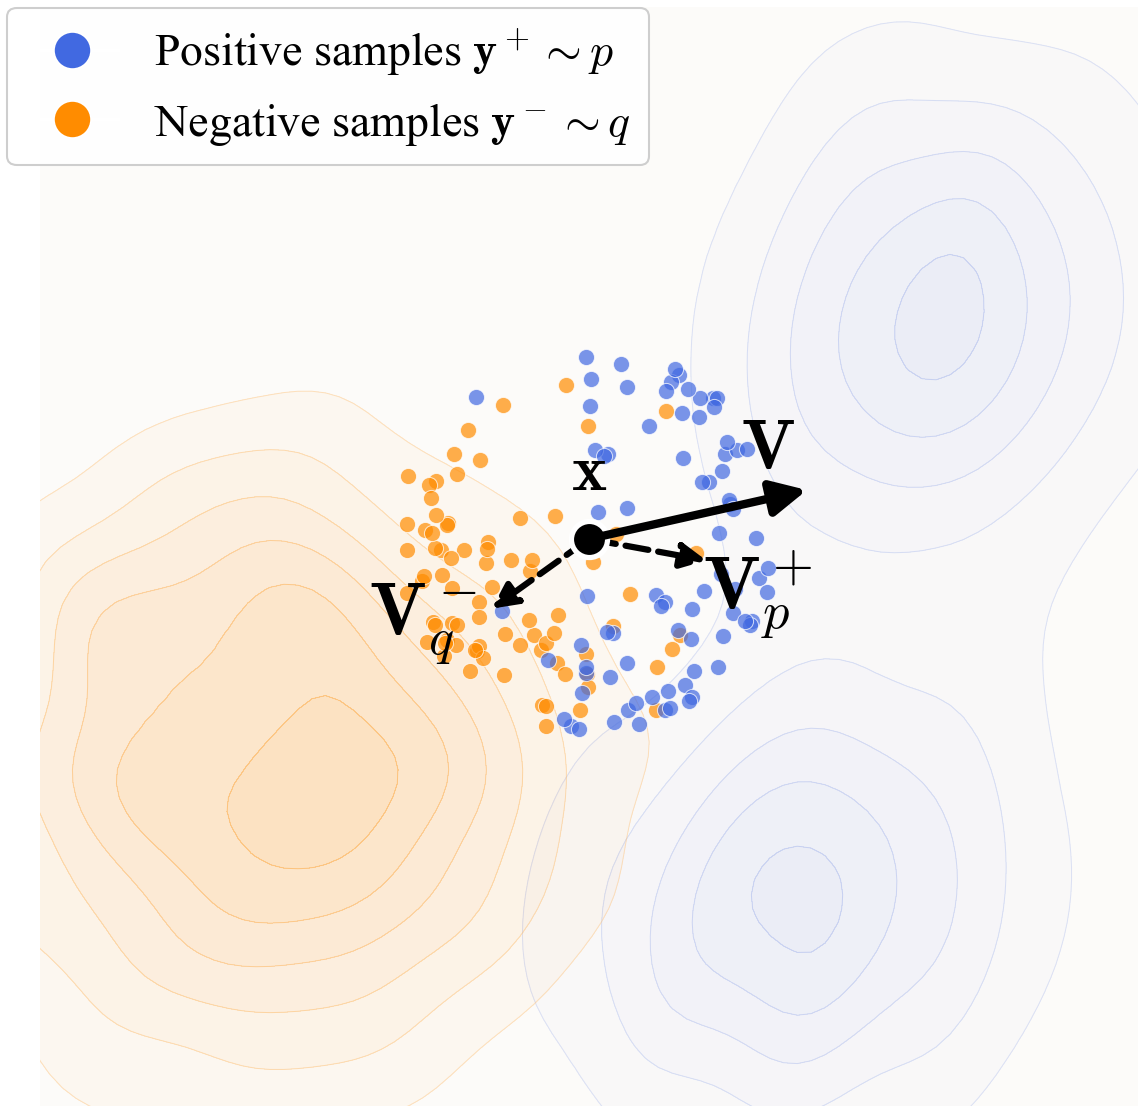
\includegraphics[width=0.9\linewidth]{figures/drift_field.png}
    \caption{\textbf{Illustration of drifting a sample.}
    A generated sample $\mathbf{x}$ (black) drifts according to a vector:
    $\V=\V^+_{p}-\V^-_{q}$. 
    Here, $\V^+_{p}$ is the mean-shift vector of the positive samples (blue) and $\V^-_{q}$ is the mean-shift vector of the negative samples (orange): see Eq.~(\ref{eq:meanshift}).
    $\x$ is attracted by $\V^+_{p}$ and repulsed by $\V^-_{q}$.
    }
    \label{fig:micro_shift}
\end{figure}
% ==============================================================

\paragraph{Kernel.}
The kernel $k(\cdot, \cdot)$ can be a function that measures the similarity. In this paper, we adopt:
\begin{equation}
\label{eq:kernel}
k(\x, \y) = \exp\left(-\frac{1}{\tau} \|\x - \y\|\right),
\end{equation}
where $\tau$ is a temperature and $\|\cdot\|$ is $\ell_2$-distance. We view $\tilde{k}(\x, \y) \triangleq\frac{1}{Z}k(\x, \y)$ as a normalized kernel, which absorbs the normalization in Eq.~(\ref{eq:VZZ}).

In practice, we implement $\tilde{k}$ using a \textit{softmax} operation, with logits given by $-\frac{1}{\tau} \|\x - \y\|$, where the softmax is taken over $\y$.
This softmax operation is similar to that of InfoNCE \cite{oord2018representation} in contrastive learning.
In our implementation, we further apply an extra softmax normalization over the set of $\{\x\}$ within a batch, which slightly improves performance in practice. This additional normalization does not alter the antisymmetric property of the resulting $\V$.

\paragraph{Equilibrium and Matched Distributions.}
Since our training loss in Eq.~(\ref{eq:train_loss}) encourages minimizing $\|\V\|^2$, we hope that $\V \approx \textbf{0}$ leads to $q\approx p$.
While this implication does not hold for arbitrary choices of $\V$, we empirically observe that decreasing the value of $\|\V\|^2$ correlates with improved generation quality. In Appendix~\ref{sec:theory_identifiability}, we provide an identifiability heuristic: for our kernelized construction, the zero-drift condition imposes a large set of bilinear constraints on $(p,q)$, and under mild non-degeneracy assumptions this forces $p$ and $q$ to match (approximately).
% In Appendix~\ref{sec:theory_identifiability}, we show that under certain assumptions and with kernelization, $\V_{p,q}\approx\mathbf{0}$ implies $q\approx p$.


% 

% ========================================
\begin{algorithm}[t]
\caption{
\textbf{Training Loss.} Note: for brevity, here the negative samples $\texttt{y\_neg}$ are from the same batch of generated data, though they can include other source of negatives.
}
\label{alg:training_code}
\begin{lstlisting}
# f: generator
# y_pos: [N_pos, D], data samples

e = randn([N, C]) # noise
x = f(e) # [N, D], generated samples
y_neg = x # reuse x as negatives

V = compute_V(x, y_pos, y_neg)
x_drifted = stopgrad(x + V)

loss = mse_loss(x - x_drifted)
\end{lstlisting}
\end{algorithm}

\paragraph{Stochastic Training.}
In stochastic training (\eg, mini-batch optimization), we estimate $\V$ by approximating the expectations in Eq.~(\ref{eq:VZZ}) with empirical means.
For each training step, we draw $N$ samples of noise $\e \sim 
p_\e$ and compute a batch of $\x=f_\theta(\e)\sim q$.
The generated samples also serve as the negative samples in the same batch, \ie, $\y^- \sim q$.
On the other hand, we sample $N_\text{pos}$ data points $\y^+ \sim p_\text{data}$. The drifting field $\V$ is computed in this batch of positive and negative samples. 
Alg.~\ref{alg:training_code} provide the pseudocode for such a training step, where \texttt{compute\_V} is given in \cref{sec:appendix_compute_V}.

\subsection{Drifting in Feature Space}
\label{subsec:feature_space}

Thus far, we have defined the objective (\ref{eq:train_loss}) directly in the raw data space. Our formulation can be extended to any feature space.
Let $\phi$ denote a feature extractor (\eg, an image encoder) operating on real or generated samples. We rewrite the loss (\ref{eq:train_loss}) in the feature space as:
\begin{equation}
\mathbb{E}\!\left[
\left\|
\phi(\x)
-
\text{\texttt{stopgrad}}\Big(
\phi(\x)
+
\V\big(\phi(\x)\big)
\Big)
\right\|^2
\right].
\label{eq:feature_space}
\end{equation}
Here, $\x=f_\theta(\e)$ is the output (\eg, images) of the generator. $\V$ is defined in the feature space: in practice, this means that
$\phi(\y^+)$ and $\phi(\y^-)$ serve as the positive/negative samples.
It is worth noting that feature encoding is a training-time operation and is not used at inference time.


This can be further extended to multiple features, \eg, at multiple scales and locations:
\begin{equation}
\sum_j\mathbb{E}\!\left[
\left\|
\phi_j(\x)
-
\text{\texttt{stopgrad}}\Big(
\phi_j(\x)
+
\V\big(\phi_j(\x)\big)
\Big)
\right\|^2
\right].
\label{eq:feature_space_multi}
\end{equation}
Here, $\phi_j$ represents the feature vectors at the $j$-th scale and/or location from an encoder $\phi$.
With a ResNet-style image encoder \cite{he2016deep}, we compute drifting losses across multiple scales and locations, which provides richer gradient information for training.


The feature extractor plays an important role in the generation of high-dimensional data.
As our method is based on the kernel $k(\cdot, \cdot)$ for characterizing sample similarities, it is desired for semantically similar samples to stay close in the feature space. This goal is aligned with self-supervised learning (\eg, \citealt{he2020momentum,chen2020simple}). 
We use pre-trained self-supervised models as the feature extractor.

\paragraph{Relation to Perceptual Loss.}
Our feature-space loss is related to perceptual loss \cite{zhang2018unreasonable} but is conceptually different. The perceptual loss minimizes: $\|\phi(\x)-\phi(\x_\text{target})\|_2^2$, that is, the regression target is $\phi(\x_\text{target})$ and requires pairing $\x$ with its target.
In contrast, our regression target in (\ref{eq:feature_space}) is
$
\phi(\x)
+
\V\big(\phi(\x)\big)
$, where the drifting is in the feature space and requires no pairing. 
In principle, our feature-space loss aims to match the pushforward distributions $\phi_\#q$ and $\phi_\#p$.

\paragraph{Relation to Latent Generation.}
Our feature-space loss is \textit{orthogonal} to the concept of generators in the latent space (\eg, Latent Diffusion \cite{rombach2022high}).
In our case, when using $\phi$,
the generator $f$ can still produce outputs in the pixel space or the latent space of a tokenizer.
If the generator $f$ is in the latent space and the feature extractor $\phi$ is in the pixel space, the tokenizer decoder is applied before extracting features from $\phi$.


\subsection{Classifier-Free Guidance}
\label{subsec:additive_guidance}

Classifier-free guidance (CFG)~\cite{ho2022classifier} improves generation quality by extrapolating between class-conditional and unconditional distributions.
Our method naturally supports a related form of guidance.


In our model, given a class label $c$ as the condition, the underlying target distribution $p$ now becomes $p_{\text{data}}(\cdot|c)$, from which we can draw positive samples: $\y^+ \sim p_{\text{data}}(\cdot|c)$.
To achieve guidance, we draw {negative} samples either from generated samples or \textit{real} samples from different classes.
Formally, the negative sample distribution is now:
\begin{equation}
\tilde{q}(\cdot|c) \triangleq (1-\gamma)\,q_\theta(\cdot|c)   + \gamma\,p_{\text{data}}(\cdot | \varnothing).
\label{eq:cfg1}
\end{equation}
Here, $\gamma \in [0, 1)$ is a mixing rate,
and $p_{\text{data}}(\cdot | \varnothing)$ denotes the \textit{unconditional} data distribution\footnotemark{}.

The goal of learning is to find $\tilde{q}(\cdot|c)=p_\text{data}(\cdot|c)$.
Substituting it into (\ref{eq:cfg1}), we obtain:
\begin{equation}
q_\theta(\cdot|c) = \alpha\, p_{\text{data}}(\cdot|c) - (\alpha - 1)\, p_{\text{data}}(\cdot | \varnothing).
\label{eq:cfg2}
\end{equation}
where $\alpha=\frac{1}{1-\gamma} \geq 1$.
This implies that $q_\theta(\cdot|c)$ is to approximate a linear combination of conditional and unconditional data distributions. This follows the spirit of original CFG.


\footnotetext{This should be the data distribution excluding the class $c$. For simplicity, we use the unconditional data distribution.}

In practice, Eq.~(\ref{eq:cfg1}) means that we sample extra negative examples from the data in $p_{\text{data}}(\cdot | \varnothing)$, in addition to the generated data. The distribution $q_\theta(\cdot|c)$ corresponds to a class-conditional network $f_\theta(\cdot | c)$, similar to common practice \cite{ho2022classifier}.
We note that, in our method, CFG is a \textit{training-time} behavior by design: the one-step (1-NFE) property is preserved at inference time.



